\documentclass[a4paper,11pt,exos]{nsi} % COMPILE WITH DRAFT
\usepackage{pifont}
\usepackage{fontawesome5}
\usepackage{hyperref}



\begin{document}
\classe{\terminale Comp}
\titre{Stat à deux variables quantitatives}
\maketitle

\tabularstyled[UGLiBlue]
\begin{tabular}{p{16.5cm}}
    \rowcolor{UGLiBlue}
    \ths Capacités attendues : \\

    \ding{111} Représenter un nuage de points.   \\
    \ding{111} Calculer les coordonnées d’un point moyen. \\
    \ding{111} Déterminer une droite de régression, à l’aide de la calculatrice, d’un logiciel ou par calcul.\\
    \ding{111} Dans le cadre d’une résolution de problème, utiliser un ajustement pour interpoler, extrapoler.\\
\end{tabular}


\vspace*{.5cm}

\subsection*{Nuage de points, ajustement}
\exo{}
Parmi les nuages de points suivants, lesquel semblent « ajustables » par une fonction reconnaissable ? Citer la fonction correspondante.
\begin{multicols}{2}
    \begin{enumerate}
        \item 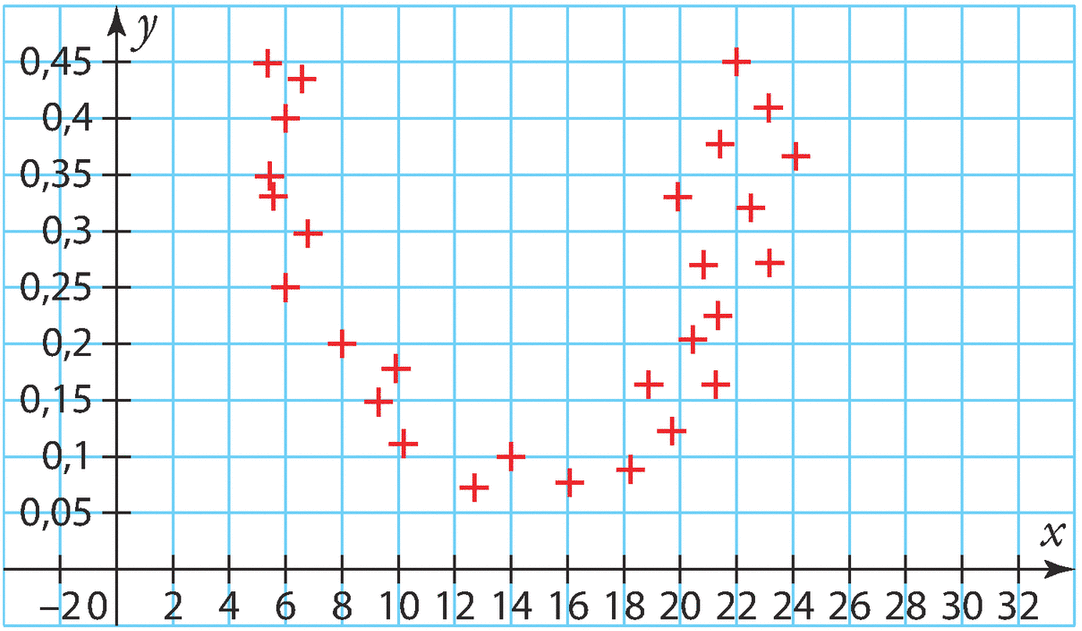
\includegraphics[width=7cm]{Ex18aSesamath.png}
        \item 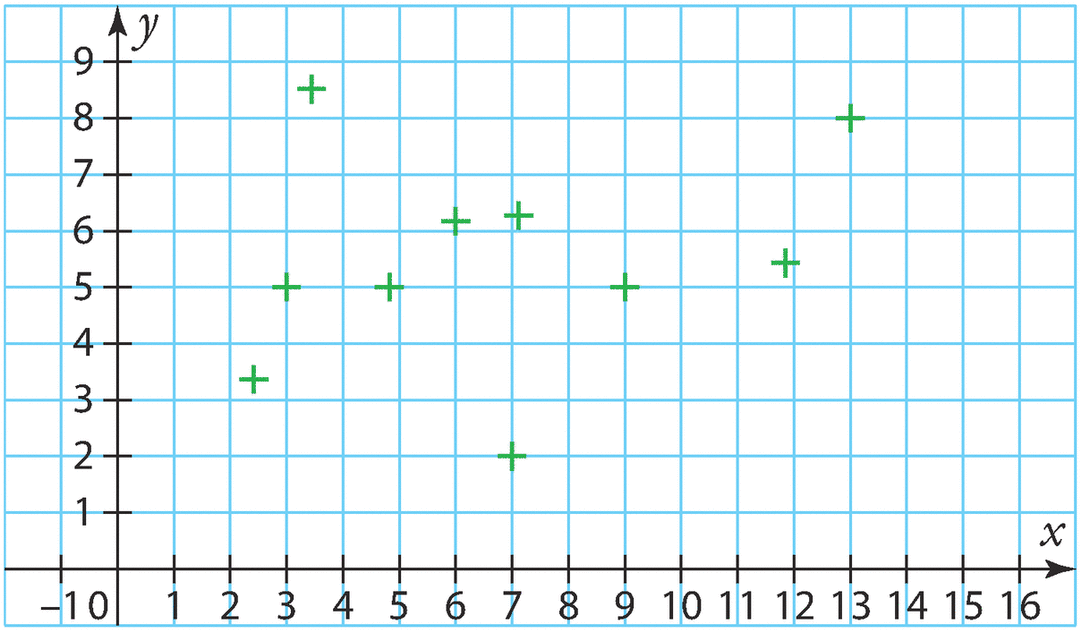
\includegraphics[width=7cm]{Ex18bSesamath.png}
        \item 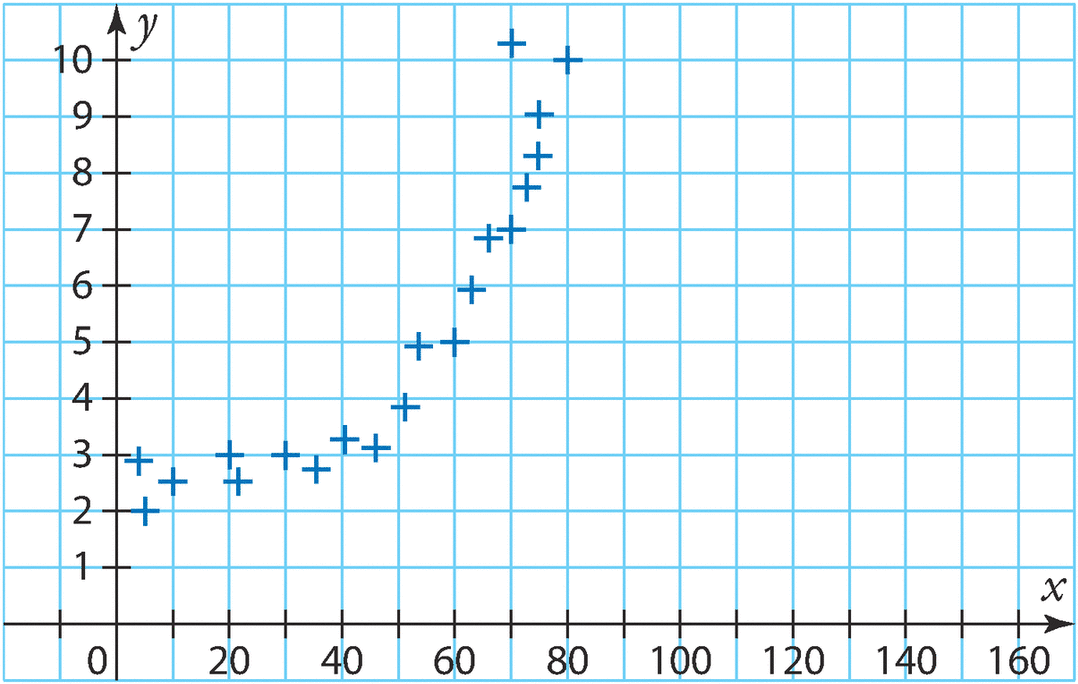
\includegraphics[width=7cm]{Ex18cSesamath.png}
        \item 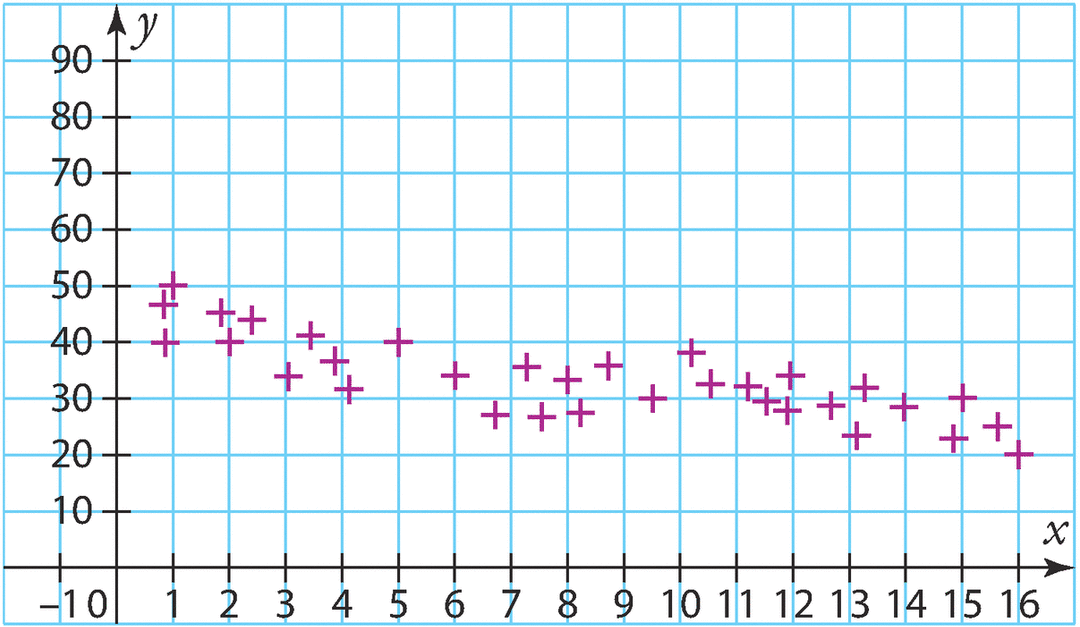
\includegraphics[width=7cm]{Ex18dSesamath.png}
    \end{enumerate}
\end{multicols}


\dleft{10.2cm}{
    \exo{}
    \begin{enumerate}
        \item Dans le nuage de points ci-contre, parmi les points A, J, O, D, K, quel point semble être le point moyen du nuage ?
        \item Peut-on trouver une corrélation entre les deux variables $x$ et $y$ de la série statistique double associée à ce nuage de points ?
    \end{enumerate}
}
{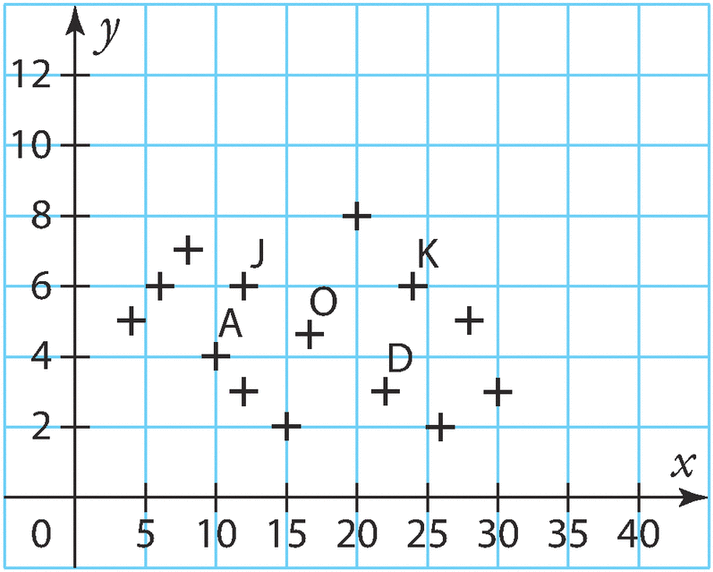
\includegraphics[width=6cm]{Ex19Sesamath.png}}

\subsection*{Exploiter un ajustement affine}


\dleft{8.2cm}{
    \exo{}
    Le graphique ci-contre présente l'évolution annuelle du nombre de gardons dans un étang depuis l'année 2017 (année 0).\\
    Le nuage de points obtenu peut être ajusté par la droite $(d)$ représentée sur le graphique.\\    
}
{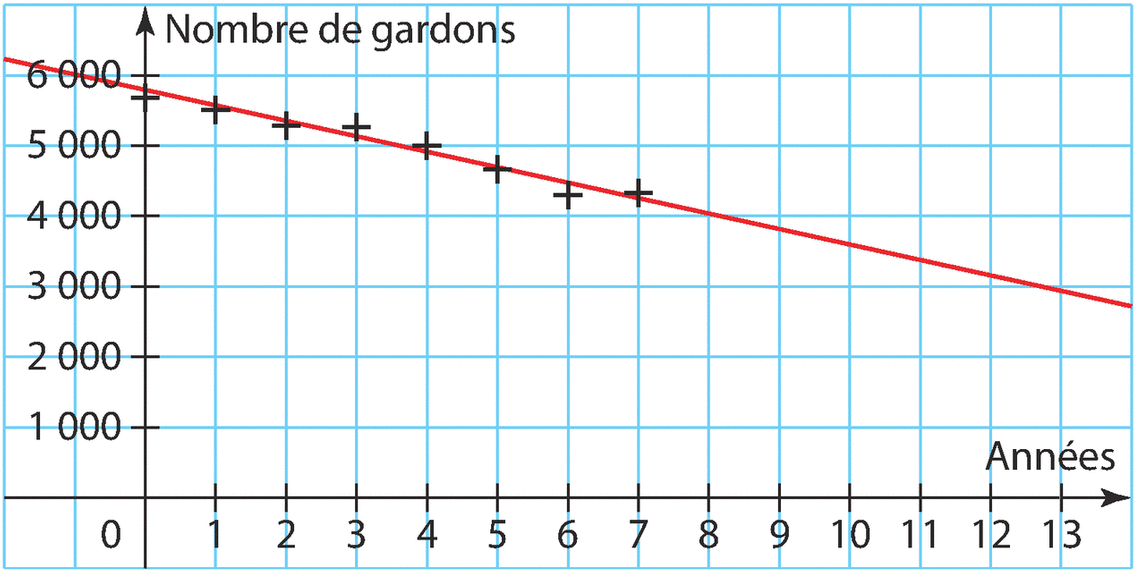
\includegraphics[width=8cm]{Ex17Sesamath.png}}
Si l'évolution continue pendant encore plusieurs années selon l'ajustement modélisé par la droite $(d)$, estimer graphiquement :
    \begin{enumerate}
        \item Le nombre de gardons dans l'étang en 2025.
        \item L'année à partir de laquelle il y aura moins de 3000 gardons dans l'étang.
    \end{enumerate}

\exo{}
La maire d'un village a fait comptabiliser le nombre de mégots ramassés annuellement dans la rue principale de sa commune entre 2020 et 2024. La variable $x_i$ correspond au rang de l'année d'observation et la variable $y_i$ au nombre, en milliers, de mégots ramassés. Voici les résultats obtenus :
\begin{center}
    \tabstyle[UGLiBlue]
    \begin{tabular}{|c|c|c|c|c|c|c|}
    \hline
    \ccell Année & 2020 & 2021 & 2022 & 2023 & 2024 & \ccell Total \\\hline
    \ccell Rang $x_i$ & 1 & 2 & 3 & 4 & 5 & 15\\\hline
    \ccell Quantité $y_i$ & 10 & 9,1 & 8,5 & 7,6 & 6,8 & 42 \\\hline
    \end{tabular}
\end{center}
\begin{enumerate}
    \item Dans un repère, on note $M_i$ le point de coordonnées $\pc{M_i}{x_i}{y_i}$ pour $i=1,2,...,5$. Représenter le nuage de points associé à cette série statistique.
    \item Calculer les coordonnées du point moyen $G$ de cette série statistique. Placer $G$ sur le graphique.
    \item On ajuste le nuage par la droite $(GM_5)$. Déterminer l'équation réduite de $(GM_5)$.
    \item En supposant que l'évolution se poursuive ainsi, estimer le nombre de mégots qui seraient ramassés dans cette rue en 2030.
\end{enumerate}

\exo{}
Le tableau ci-dessous donne l'évolution du montant net du SMIC (Salaire Minimum Interprofessionnel de Croissance) mensuel, en euros, entre 2000 et 2005. 
\begin{center}
    \tabstyle[UGLiBlue]
    \begin{tabular}{|c|c|c|c|c|c|c|}
    \hline
    \ccell Année & 2000 & 2001 & 2002 & 2003 & 2004 & 2005 \\\hline
    \ccell Rang $x_i$ & 1 & 2 & 3 & 4 & 5 & 6\\\hline
    \ccell Montant $y_i$ & 842 & 874 & 903 & 934 & 985 & 1039\\\hline
    \end{tabular}
\end{center}
\begin{enumerate}
    \item Représenter, dans un repère, le nuage de points $\pc{M_i}{x_i}{y_i}$ associé à cette série statistique et placer le point moyen $G$.
    \item Déterminer l'équation de la droite $(GM_5)$.
    \item En 2025, le SMIC net mensuel est de 1426 €. Comparer ce montant à celui extrapolé avec la droite précédente.
\end{enumerate}


\subsection*{Méthode des moindres carrés}

\dleft{10cm}{    
    \exo{}
    Edwin affirme « La méthode des moindres carrés minimise la somme des $M_iH_i^2$, comme représenté ci-contre. »\\
    A-t-il raison ?
}
{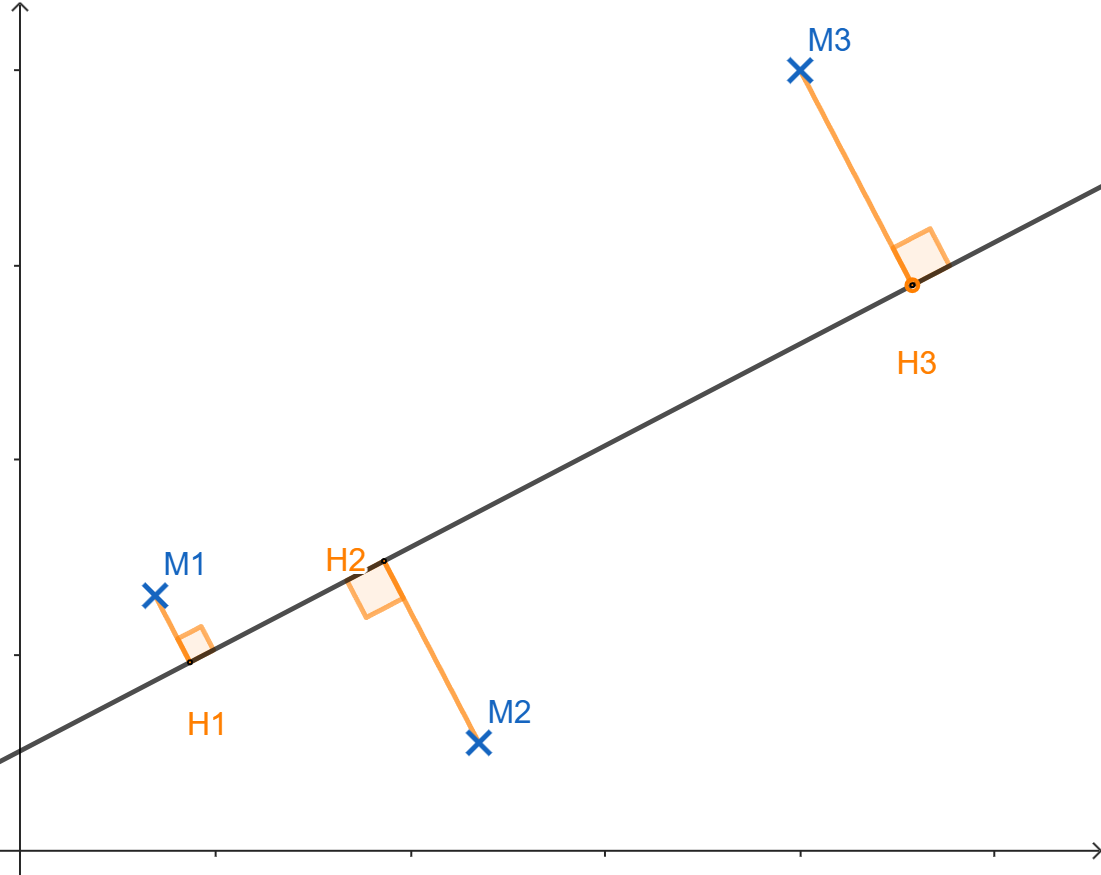
\includegraphics[width=6cm]{Ex17Hyperbole.png}}

\exo{}
Dans un repère orthogonal, le point $\pc{G}{5}{4}$ est le point moyen d'un nuage de points.\\
Martha affirme « La droite d'ajustement affine associée à ce nuage obtenue par la méthode des moindres carrés a pour équation $y=-2x+1$. »\\
Peut-elle avoir raison ?


\exo{}
Le tableau ci-dessous donne la masse $x$ (en kg) et la taille $y$ (en cm) d'un enfant, relevées par son médecin lors de six visites médicales.
\begin{center}
    \tabstyle[UGLiBlue]
    \begin{tabular}{|c|c|c|c|c|c|c|}
    \hline
    \ccell Masse $x_i$ (en kg)& 4 & 5,4 & 10,2 & 11 & 12,6 & 19,8\\\hline
    \ccell Taille $y_i$ (en cm)& 53 & 61 & 72 & 78 & 94 & 113\\\hline
    \end{tabular}
\end{center}
On veut réaliser un ajustement affine de cette série par la méthode des moindres carrés.

\begin{enumerate}
    \item Calculer les valeurs moyennes $\overline{x}$ et $\overline{y}$ des deux séries $(x_i)$ et $(y_i)$.
    \item Compléter le tableau suivant :
    \begin{center}
        \renewcommand{\arraystretch}{1.5}
        \tabstyle[UGLiBlue]
        \begin{tabular}{|c|c|c|c|c|c|c|}
        \hline
        \ccell Masse $x_i$ (en kg)& 4 & 5,4 & 10,2 & 11 & 12,6 & 19,8\\\hline
        \ccell Taille $y_i$ (en cm)& 53 & 61 & 72 & 78 & 94 & 113\\\hline
        \ccell Écarts $x_i - \overline{x}$ & $\qquad$  &  $\qquad$ & $\qquad$  & $\qquad$  & $\qquad$  &  $\qquad$ \\\hline
        \ccell Écarts $y_i - \overline{y}$ &   &   &   &   &   &   \\\hline
        \ccell Produit des écarts $(x_i - \overline{x})(y_i - \overline{y})$ &   &   &   &   &   &   \\\hline
        \ccell Carré des écarts $(x_i - \overline{x})^2$ &   &   &   &   &   &   \\\hline
        \end{tabular}
    \end{center}
    En déduire covariance entre les deux séries $\mathrm{Cov}(x,y)$ et la variance $\mathrm{Var}(x)$ de la série $(x_i)$.
    \item En déduire l'équation de la droite de d'ajustement affine $(d)$ de la série $(x_i,y_i)$ par la méthode des moindres carrés.
    \item Représenter le nuage de points $\pc{M_i}{x_i}{y_i}$ et la droite $(d)$ dans un repère orthonormé.
    \item Quelle estimation peut-on faire de la taille de cette enfant lorsqu'il pèsera 25 kg ?
\end{enumerate}

\exo{}
On a relevé à certaines latitudes $x_i$ (en degrés) la température $y_i$ (en °C) à la surface de la mer. Voici les résultats obtenus :
\begin{center}
    \tabstyle[UGLiBlue]
    \begin{tabular}{|c|c|c|c|c|}
    \hline
    \ccell Latitude $x_i$ (en °)& $-$45 & $-$20 & 0 & 30 \\\hline
    \ccell Température $y_i$ (en °C)& 12,2 & 12,9 & 13,4 & 14,1 \\\hline
    \end{tabular}
\end{center}
\begin{enumerate}
    \item Calculer la covariance entre les deux séries $\mathrm{Cov}(x,y)$ et la variance $\mathrm{Var}(x)$ de la série $(x_i)$.
    \item En déduire l'équation de la droite de d'ajustement affine $(d)$ de la série $(x_i,y_i)$ par la méthode des moindres carrés.
    \item Représenter le nuage de points $\pc{M_i}{x_i}{y_i}$ et la droite $(d)$ dans un repère orthonormé.
\end{enumerate}

\exo{ \faCalculator} % Ex24 Sesamath
Sous des conditions de température et de volume constants, on étudie la pression et la quantité de matière d'un gaz. Les résultats sont donnés dans le tableau ci-dessous :
\begin{center}
    \tabstyle[UGLiBlue]
    \begin{tabular}{|c|c|c|c|c|}
    \hline
    \ccell Nombre de moles $x_i$ & 0 & 10 & 20 & 30\\\hline
    \ccell Pression $y_i$ (en kPa) & 0 & 46 & 98 & 145\\\hline
    \end{tabular}
\end{center}
\begin{enumerate}
    \item Dans un reprère orthonormé, représenter le nuage de points $\pc{M_i}{x_i}{y_i}$ et vérifier qu'il peut être ajusté par une droite.
    \item \faCalculator \hspace*{.2cm} Déterminer l'équation réduite de la droite $(d)$ d'ajustement affine de la série $(x_i,y_i)$ par la méthode des moindres carrés et le coefficient de corrélation linéaire.
    \item Représenter la droite $(d)$ dans le repère.
    \item Quel serait la pression du gaz si l'on avait 50 moles ?
    \item Combien de moles aurait-on si le gaz avait une pression de 200 kPa ?
\end{enumerate}

\exo{ \faCalculator}
On considère la série statistique à deux variables $(x,y)$ donnée par le tableau suivant :
\begin{center}
    \tabstyle[UGLiBlue]
    \begin{tabular}{|c|c|c|c|c|c|}
    \hline
    \ccell Valeurs $x_i$ & $-$11 & $-$3 & 2 & 0 & $-$5\\\hline
    \ccell Valeurs $y_i$ & 1100 & 1000 & 900 & 950 & 1050\\\hline
    \end{tabular}
\end{center}
\begin{enumerate}
    \item Dans un repère orthogonal, représenter le nuage de points $\pc{M_i}{x_i}{y_i}$ et vérifier qu'il peut être ajusté par une droite.
    \item \faCalculator \hspace*{.2cm} Déterminer l'équation réduite de la droite $(d)$ d'ajustement affine de la série $(x_i,y_i)$ par la méthode des moindres carrés et le coefficient de corrélation linéaire.
    \item Représenter la droite $(d)$ dans le repère.
\end{enumerate}

\newpage
\subsection*{Ajustement se ramenant par changement de variable à un ajustement affine}
\exo{}%Sesamath 26 p 237
On injecte un médicament dans le sang d'une patiente en lui faisant une piqûre en intraveineuse.\\
La concentration $y_i$ de ce médicament dans le sang, en micogrammes par millilitres est relevée à différents instants $x_i$ (en heures) après la piqûre. Voici les résultats obtenus :
\begin{center}
    \tabstyle[UGLiBlue]
    \begin{tabular}{|c|c|c|c|c|c|c|}
    \hline
    \ccell Temps $x_i$ (en h) & 0 & 1 & 2 & 4 & 6 & 10\\\hline
    \ccell Concentration $y_i$ (en $\mu g/mL$) & 90 & 65 & 45 & 23 & 12 & 4\\\hline
    \end{tabular}
\end{center}
\begin{enumerate}
    \item Représenter le nuage de points $\pc{M_i}{x_i}{y_i}$ sur la calculatrice et vérifier qu'il peut être ajusté par une fonction exponentielle décroissante.
    \item On pose $y'_i=\ln(y_i)$ pour tout entier $i$ de 1 à 6.\\
    Compléter le tableau suivant :
    \begin{center}
        \tabstyle[UGLiBlue]
        \begin{tabular}{|c|c|c|c|c|c|c|}
        \hline
        \ccell $x_i$ & 0 & 1 & 2 & 4 & 6 & 10\\\hline
        \ccell $y_i$ & 90 & 65 & 45 & 23 & 12 & 4\\\hline
        \ccell $y'_i$ & \hspace*{1cm}  & \hspace*{1cm}  & \hspace*{1cm}  &  \hspace*{1cm} & \hspace*{1cm}  &  \hspace*{1cm} \\\hline
        \end{tabular}
    \end{center}
    \item Représenter le nuage de points $\pc{M_i}{x_i}{y'_i}$ sur la calculatrice et vérifier qu'il peut être ajusté par une droite.
    \item Déterminer l'équation de la droite $(d)$ d'ajustement affine de la série $(x_i,y'_i)$ par la méthode des moindres carrés.
    \item En déduire une approximation de la concentration $y$ en fonction du temps $x$.
\end{enumerate}
\vspace*{.1cm}


\dleft{7.3cm}{
    \exo{} %Sesamath 50 p 242
    Le document ci-contre donne les valeurs moyennes de la distance de réaction et de la distance de freinage selon la vitesse d'un véhicule, sur route sèche, de jour et dans des conditions de visibilité normales.
}
{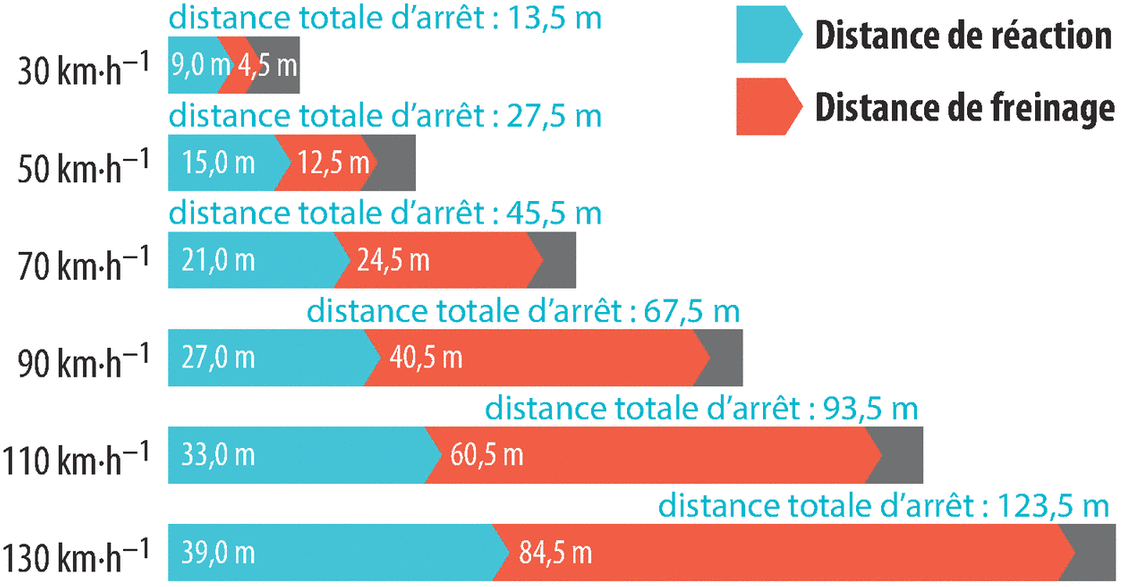
\includegraphics[width=9cm]{Ex50p242Sesamath.png}}

\subsubsection*{Partie A : Étude de la série statistique à deux variables : vitesse $x$ et distance de réaction $y$}
\begin{enumerate}
    \item Construire dans un repère orthonormé le nuage de points correspondant à la série statistique $(x,y)$ où $x$ représente la vitesse du véhicule en km.h$^{-1}$ et $y$ la distance de réaction en mètres.\\
    Vérifier que la forme du nuage de points invite à réaliser un ajustement affine.
    \item Déterminer à l'aide de la calculatrice l'équation de la droite d'ajustement affine du nuage obtenu par la méthode des moindres carrés.
    \item Selon cet ajustement :
    \begin{enumalph}
        \item Estimer la distance de réaction d'un véhicule roulant, en excès de vitesse, à 140 km.h$^{-1}$.
        \item Estimer la vitesse à laquelle un véhicule doit rouler pour que la distance de réaction soit inférieure à 3 m.
    \end{enumalph}
\end{enumerate}
\subsubsection*{Partie B : Étude de la série statistique à deux variables : vitesse $x$ et distance de freinage $y'$}
\begin{enumerate}
    \item Construire dans un repère orthonormé le nuage de points correspondant à la série statistique $(x,y')$ où $x$ représente la vitesse du véhicule en km.h$^{-1}$ et $y'$ la distance de freinage en mètres.\\
    Vérifier que la forme du nuage de points invite à réaliser un ajustement affine.
    \item On considère que ce nuage de points peut être ajusté par une parabole d'équation $y' = ax^2$ où $a$ est un réel non nul.
    \begin{enumalph}
        \item On pose $z=\sqrt{y'}$. Compléter le tableau suivant :
        \begin{center}
            \tabstyle[UGLiBlue]
            \begin{tabular}{|c|c|c|c|c|c|c|}
            \hline
            \ccell Vitesse $x$ (en km.h$^{-1}$) & 30 & 50 & 70 & 90 & 110 & 130\\\hline
            \ccell Distance de freinage $y'$ (en m) & 4,5 & 12,5 & 24,5 & 40,5 & 60,5 & 84,5\\\hline
            \ccell $z=\sqrt{y'}$  & \hspace*{1cm}  & \hspace*{1cm}  & \hspace*{1cm}  &  \hspace*{1cm} & \hspace*{1cm} & \hspace*{1cm}\\\hline
            \end{tabular}
        \end{center}
        \item À l'aide de la calculatrice, déterminer l'équation de la droite de regression de $z$ en $x$.
        \item En déduire une approximation de la distance de freinage $y'$ en fonction de la vitesse $x$.
    \end{enumalph}
    \item Pour les questions suivantes, on admet que la fonction définie sue $\fio{0}{+\infty}$ par $f(x)=\dfrac{x^2}{200}$ est une bonne modélisation de la distance de freinage $y'$ en fonction de la vitesse $x$.
    \begin{enumalph}
        \item Estimer la distance de freinage d'un véhicule roulant, en excès de vitesse, à 140 km.h$^{-1}$.
        \item À l'aide de la partie A, estimer la distane totale d'arrêt pour un véhicule roulant en excès de vitesse à 140 km.h$^{-1}$.
    \end{enumalph}
\end{enumerate}

\exo{} % Sesamath 49 p 242
En 2020, un lycée décide de créer un club d'échecs.\\
Le nombre d'adhérents chaque année depuis 2020 est donné dans le tableau ci-dessous :
\begin{center}
    \tabstyle[UGLiBlue]
    \begin{tabular}{|c|c|c|c|c|}
    \hline
    \ccell Année & 2020 & 2021 & 2022 & 2023\\\hline
    \ccell Rang $x_i$ & 1 & 2 & 3 & 4 \\\hline
    \ccell Nombre d'adhérents $y_i$ & 9 & 15 & 22 & 31\\\hline
    \end{tabular}
\end{center}
\begin{enumerate}
    \item On considère la série statistique à deux variables $(x,y)$ donnée par le tableau ci-dessus.\\
    Déterminer le coefficient de corrélation linéaire $r_1$ de cette série statistique $(x,y)$.
    \item On pose $z=\ln (y)$ et on considère la série statistique à deux variables $(x,z)$.\\
    Déterminer le coefficient de corrélation linéaire $r_2$ de cette série statistique $(x,z)$.
    \item Depuis la création du club, la présidente espère une progression exponentielle du nombre d'adhérents. Pour ces quatre premières années, peut-on dire que ses espérances sont satisfaites ?
    \item En 2024, une grande campage de publicité a été organisée au lycée. Le nombre de participants totalisés à la fin de l'année est de 44.\\
    La présidente du club, après avoir observé l'ensemble des données de 2020 à 2024, affirme dans son discours de fin d'année : « Si on continue sur cette lancée, nous serons au moins 67 adhérents l'année prochaine ! »\\
    Qu'en pensez-vous ?
\end{enumerate}
\end{document}